%\RequirePackage{fix-cm}
\documentclass{llncs}
%\smartqed  % flush right qed marks, e.g. at end of proof
\usepackage{stmaryrd}
%\usepackage{citesort} % removed because it clashes with the hyperref package
\usepackage{bussproofs}
\usepackage{turnstile}
\usepackage{amssymb}
\usepackage{latexsym}
\setcounter{tocdepth}{3}
\usepackage{graphicx}
\usepackage{url}
\usepackage{amsmath}
\usepackage{listings}
\usepackage{subfig}
\usepackage{pgf}
\usepackage{tikz}
\usetikzlibrary{arrows,shapes,snakes,automata,backgrounds,petri}
\usepackage[latin1]{inputenc}
\usepackage{float}
\usepackage{amssymb}
\usepackage{wrapfig}
\usepackage{lscape}
\usepackage[counterclockwise]{rotating}
\usepackage{hyperref}

   
\usepackage{ifthen}
\usepackage{amssymb}
\newboolean{showcomments}
\setboolean{showcomments}{true}
\ifthenelse{\boolean{showcomments}}
  {\newcommand{\mynote}[2]{
    \fbox{\bfseries\sffamily\scriptsize#1}
    {\small$\blacktriangleright$\textsf{\emph{#2}}$\blacktriangleleft$}
   }
  }
  {\newcommand{\mynote}[2]{}
  }
\newcommand\laurie[1]{\mynote{Laurie}{#1}}
\newcommand\richard[1]{\mynote{Richard}{#1}}

\newcommand{\MAY}[2]{\langle #1 \rangle #2}
\newcommand{\NEG}[1]{\mathsf{neg}(#1)}
\newcommand{\AND}{\land}

\lstnewenvironment{code}
    {\lstset{}%
      \csname lst@SetFirstLabel\endcsname}
    {\csname lst@SaveFirstLabel\endcsname}
    \lstset{
      basicstyle=\small\ttfamily,
      flexiblecolumns=false,
      basewidth={0.5em,0.45em},
      literate={+}{{$+$}}1 {/}{{$/$}}1 {*}{{$*$}}1 {=}{{$=$}}1
               {>}{{$>$}}1 {<}{{$<$}}1 {\\}{{$\lambda$}}1
               {\\\\}{{\char`\\\char`\\}}1
               {->}{{$\rightarrow$}}2 {>=}{{$\geq$}}2 {<-}{{$\leftarrow$}}2
               {<=}{{$\leq$}}2 {=>}{{$\Rightarrow$}}2 
               {\ .}{{$\bigcirc$}}2 {\ .\ }{{$\bigcirc$}}2
               {>>}{{>>}}2 {>>=}{{>>=}}2
               {|}{{$\mid$}}1               
    }

\newtheorem{mycase}{Case}
\newtheorem{subcase}{Case}
\numberwithin{subcase}{mycase}


% Dot
\def\fDot {\ast}
% Bang
\def\fBang {\ ! \ }
% Or
\def\fOr {\ | \ }

% Turnstiles with subscripts
\def\judgeX {\sststile{\mathrm{X}}{}}
\def\judgeY {\sststile{\mathrm{Y}}{}}
\def\judge {\sststile{\mathrm{}}{}}

\EnableBpAbbreviations


\begin{document}

\title {Cathoristic logic: A logic for capturing inferences between atomic sentences\thanks{The present version is an extended abstract of \cite{Evans:catlogLONG}.}}
\titlerunning{Cathoristic logic}
\author{Richard Prideaux Evans\inst{1} \and  Martin Berger\inst{2}}
\authorrunning{Prideaux Evans and Berger}
\institute {Richard Prideaux Evans, Imperial College, \email{richardevans@google.com}
  \and
 Martin Berger, University of Sussex, \email{M.F.Berger@sussex.ac.uk}.}
\date{Received: date / Accepted: date}


\bibliographystyle{abbrv} 
\maketitle

\begin{abstract}
Eremic Logic is a simple modal logic for capturing inferences between ``atomic'' sentences. 
It is the only Hennessy-Milner style logic satisfying the Hennessy-Milner theorem that has a linear-time decision procedure.
It has been put to use in an industrial application, as the representational core of a new logic programming language. The resulting code is shorter, less error-prone, and more efficient than the corresponding code in traditional predicate logic.
\end{abstract}

\section{Introduction}\label{introduction}

Natural language is full of incompatible alternatives.
If Pierre is the current king of France, then nobody else can simultaneously fill that role.
A traffic light can be green, amber or red - but it cannot be more than one colour at a time.
Mutual exclusion is a natural and ubiquitous concept.
\FOL{} can represent mutually exclusive alternatives, of course.
To say that Pierre is the only king of France, we can write, following Russell:
\[
king(france, pierre) \land \forall x . (king(france, x) \rightarrow x = pierre).
\]
To say that a particular traffic light, $tl$, is red - and red is its only colour - we could write:
\[
colour(tl, red) \land \forall x . colour(tl, x) \rightarrow x = red.
\]
In this approach, incompatibility is a \emph{derived} concept, reduced to 
a combination of universal quantification and identity.  
\FOL{}, in other words, uses relatively complex machinery to express a
simple concept:
\begin{itemize}

\item Quantification's complexity comes from the
  rules governing the distinction between free
  and bound variables.
  
\item Identity's complexity comes from the infinite collection of axioms required to formalise the
  indiscernibility of identicals.

\end{itemize}

\NI The costs of quantification and identity, such as a larger proof
search space, have to be borne every time one expresses a sentence that excludes others - even
though incompatibility does not, prima facie, appear to have anything to do
with the free/bound variable distinction, or require the full power of 
the identity relation.

This paper introduces an alternative approach, where
exclusion is expressed directly, as a first-class concept.
 \Cathoristic{}\footnote{``Cathoristic'' comes from the Greek
  $\kappa \alpha \theta o \rho \acute{\i} \zeta \epsilon i \nu$: to impose narrow
  boundaries. We are grateful to Tim Whitmarsh for suggesting this
  word.} is the simplest logic we could find in which incompatible
statements can be expressed.  
It is a multi-modal logic, a variant of Hennessy-Milner logic,
that replaces negation with a new logical primitive
\[
   !A
\]
pronounced \emph{tantum}\footnote{``Tantum'' is Latin for ``only''.}
$A$. Here $A$ is a finite set of alternatives, and $!A$ says that the
alternatives in $A$ exhaust all possibilities.  For example:
\begin{eqnarray*}
\fBang \{green, amber, red\}
\end{eqnarray*}
states that nothing but $green$, $amber$ or $red$ is possible.  Our
logic uses modalities to state facts, for example $\MAY{amber}{}$
expresses that $amber$ is currently the case.  The power of the logic
comes from the conjunction of modalities and tantum. For example
\[
   \MAY{amber}{}\ \AND\ !\{green, amber, red\} 
\]
expresses that $amber$ is currently the case and $red$ as well as
$green$ are the only two possible alternatives to $amber$.  Any
statement that exceeds what tantum $A$ allows, like
\[
   \MAY{blue} \ \AND\ !\{green, amber, red\},
\]
is necessarily false.  When the only options are green, amber, or red,
then blue is not permissible.  Now to say that Pierre is the only king
of France, we write:
\[
\MAY{king}\MAY{france}(\MAY{pierre} \land \fBang \{pierre\}).
\]
Crucially, \cathoristic{}'s representation involves no
universal quantifier and no identity relation.  It is a purely
propositional formulation.  To say that the traffic
light is currently red, and red is its only colour, we write:
\[
\MAY{tl} \MAY{colour} (\MAY{red} \land !\{red\}).
\]
This is simpler, both in terms of representation length and
computational complexity, than the formulation in \fol{} given on the
previous page.
%% \[
%% colour(tl, red) \land \forall x . colour(tl, x) \rightarrow x = red
%% \]
Properties changing over time can be expressed by adding extra
modalities that can be understood as time-stamps.  To say that that
the traffic light was red at time $t_1$ and amber at time $t_2$, we
can write:
\[
   \MAY{tl} \MAY{colour} (\MAY{t_1} (\MAY{red} \land !\{red\}) \land \MAY{t_2} (\MAY{amber} \land !\{amber\}))
\]
Change over time can be expressed in first-order logic with bounded
quantification - but modalities are succinct and avoid introducing
bound variables.

Having claimed that incompatibility is a natural logical concept, not
easily expressed in first-order logic\footnote{We will precisify this
  claim in later sections; (1) first-order logic's representation of
  incompatibility is longer in terms of formula length than
  \cathoristic{}'s (see Section \ref{incompatiblepredicatesinfol});
  and (2) logic programs in \cathoristic{} can be optimised to run
  significantly faster than their equivalent in \fol{} (see Section
  \ref{optimizingpreconditions}).}, we will now argue the following:

\begin{itemize}

\item Incompatibility is conceptually prior to negation.

\item Negation arises as the weakest form of incompatibility.

\end{itemize}

\subsection{Material incompatibility and negation}

\NI Every English speaker knows that
\begin{quote}
``Jack is alive'' is incompatible with ``Jack is dead''
\end{quote}

\NI But \emph{why} are these sentences incompatible? The orthodox
position is that these sentences are incompatible because of the
following general law:
\begin{quote}
If someone is alive, then it is not the case that they are dead
\end{quote}
Recast in first-order logic:
\[
\forall x. ( alive(x) \IMPLIES \neg dead(x) ).
\]

\NI In other words, according to the orthodox position, the
incompatibility between the two particular sentences depends on a
general law involving universal quantification, implication and
negation.

Brandom \cite{brandom2} follows Sellars in proposing an alternative explanation: ``Jack
is alive'' is incompatible with ``Jack is dead'' because ``is alive''
and ``is dead'' are \emph{materially incompatible} predicates.  They
claim we can understand incompatible predicates even if we do
not understand universal quantification or negation.  
Material incompatibility is conceptually prior to logical negation.

Imagine, to make this vivid, a primitive people speaking a primordial
language of atomic sentences\footnote{In this paper, we define a sentence as \emph{atomic} if it does
  not contain another sentence as a syntactic constituent.}. These people can express sentences
that \emph{are} incompatible.  But they cannot express \emph{that}
they are incompatible.  They recognise when atomic sentences are
incompatible, and see that one sentence entails another - but their
behaviour outreaches their ability to articulate it.

Over time, these people \emph{may} advance to a more sophisticated
language where incompatibilities are made explicit, using a negation
operator - but this is a later (and optional) development:
\begin{quote}
[If negation is added to the language], it lets one say that two
claims are materially incompatible:``If a monochromatic patch is red,
then it is not blue.'' That is, negation lets one make explicit in the
form of claims - something that can be said and (so) thought - a
relation that otherwise remained implicit in what one practically did,
namely treat two claims as materially
incompatible\footnote{\cite{brandom} pp.47-48}.
\end{quote}

\NI But before making this optional
explicating step, our primitive people understand incompatibility
without understanding negation.  If this picture of our primordial
language is coherent, then material incompatibility is conceptually
independent of logical negation.

Now imagine a modification of our primitive linguistic practice in
which no sentences are ever treated as incompatible.  If one person
says ``Jack is alive'' and another says ``Jack is dead'', nobody
counts these claims as \emph{conflicting}.  The native speakers never
disagree, back down, retract their claims, or justify them. They just
say things.  Without an understanding of incompatibility, and the
variety of behaviour that it engenders, we submit (following Brandom)
that there is insufficient richness in the linguistic practice for
their sounds to count as assertions.  Without material
incompatibility, their sounds are just \emph{barks}.
\begin{quote}

  Suppose the reporter's differential responsive dispositions to call
  things red are matched by those of a parrot trained to utter the
  same noises under the same stimulation. What practical capacities of
  the human distinguish the reporter from the parrot? What, besides
  the exercise of regular differential responsive dispositions, must
  one be able to \emph{do}, in order to count as having or grasping
  \emph{concepts}? ... To grasp or understand a concept is, according
  to Sellars, to have practical mastery over the inferences it is
  involved in... The parrot does not treat ``That's red'' as
  incompatible with ``That's green''\footnote{\cite{brandom2}
    pp.88-89, our emphasis.}.
\end{quote}

\NI If this claim is also accepted, then material incompatibility is
not just conceptually \emph{independent} of logical negation, but
conceptually \emph{prior}.  

\subsection{Negation as the minimal incompatible}

In \cite{brandom2} and \cite{brandom}, Brandom describes 
logical negation as a limiting form of material incompatibility:
\begin{quote}
Incompatible sentences are Aristotelian \emph{contraries}. A sentence
and its negation are \emph{contradictories}. What is the relation
between these? Well, the contradictory is a contrary: any sentence is
incompatible with its negation. What distinguishes the contradictory
of a sentence from all the rest of its contraries? The contradictory
is the \emph{minimal} contrary: the one that is entailed by all the
rest. Thus every contrary of ``Plane figure $f$ is a circle'' - for
instance ``$f$ is a triangle'', ``$f$ is an octagon'', and so on -
entails ``$f$ is \emph{not} a circle''.
\end{quote}

\NI If someone asserts that it is not the case that Pierre is the (only) King of France,
we have said very little.  There are so many different ways in which
it could be true:
\begin{itemize}
\item
The King of France might be Jacques
\item
The King of France might be Louis
\item
...
\item
There may be no King of France at all
\item
There may be no country denoted by the word ``France''
\end{itemize}
Each of these concrete propositions is incompatible with Pierre being the King of France.
To say ``It is not the case that the King of France is Pierre'' is just to claim that one of these indefinitely many concrete possibilities is true.
Negation is just the logically weakest form of incompatibility.

In the rest of this paper, we assume - without further argument - that material incompatibility is conceptually prior to logical negation.
We develop a simple
 modal logic to articulate Brandom's intuition: a language, without negation, in which we can nevertheless make incompatible claims.

\subsection{Inferences between atomic sentences}
\label{intrasentential}
So far, we have justified the claim that incompatibility is a
fundamental logical concept by arguing that incompatibility is
conceptually prior to negation.  Now incompatibility is an inferential
relation between \emph{atomic sentences}.  In this subsection, we
shall describe \emph{other} inferential relations between atomic
sentences - inferential relations that \fol{} cannot articulate (or
can only do so awkwardly), but that \cathoristic{} handles naturally.

The \emph{atomic sentences} of a natural language can be
characterised as the sentences which do not contain any other
sentences as constituent parts\footnote{Compare Russell \cite{russell}
  p.117: ``A sentence is of atomic form when it contains no logical
  words and no subordinate sentence''. We use a broader notion of
  atomicity by focusing solely on whether or not it contains a
  subordinate sentence, allowing logical words such as ``and'' \emph{as long
  as they are conjoining noun-phrases} and not sentences.}.  According
to this criterion, the following are atomic:

\begin{itemize}

\item Jack is alive
\item Jack loves Jill
\end{itemize}

\NI The following is not atomic:

\begin{quote}
  Jack is alive and Jill is dead
\end{quote}

\NI because it contains the complete sentence ``Jack is alive'' as a
syntactic constituent.  Note that, according to this criterion, the
following \emph{is} atomic, despite using ``and'':

\begin{quote}
  Jack loves Jill and Joan
\end{quote}

\NI Here, ``Jack loves Jill'' is not a syntactic constituent\footnote{To see that ``Jack loves Jill'' is not a constituent of ``Jack loves Jill and Joan'', observe that ``and'' conjoins constituents of the \emph{same syntactic type}. But ``Jack loves Jill'' is a sentence, while ``Joan'' is a noun. Hence the correct parsing is ``Jack (loves (Jill and Joan))'', rather than ``(Jack loves Jill) and Joan''.}.

There are many types of inferential relations between atomic
sentences of a natural language.  For example:

\begin{itemize}

\item ``Jack is alive'' is incompatible with ``Jack is dead''
\item ``Jack loves Jill'' implies ``Jack loves''
\item ``Jack walks slowly'' implies ``Jack walks''
\item ``Jack loves Jill and Joan'' implies ``Jack loves Jill''
\item ``Jack is wet and cold'' implies ``Jack is cold''

\end{itemize}

\NI The first of these examples involves an incompatibility relation,
while the others involve entailment relations.  A key question this
paper seeks to answer is: what is the simplest logic that can capture
these inferential relations between atomic sentences?

\subsection{Wittgenstein's vision of a logic of elementary propositions}

\NI In the \emph{Tractatus} \cite{wittgenstein-tractatus}, Wittgenstein
claims that the world is a set of atomic sentences in an idealised
logical language.  Each atomic sentence was supposed to be
\emph{logically independent} of every other, so that they could be
combined together in every possible permutation, without worrying
about their mutual compatibility.
But already there were doubts and problem cases.  He was aware that
certain  statements seemed atomic, but did not seem logically
independent:

\begin{quote}
  For two colours, e.g., to be at one place in the visual field is
  impossible, and indeed logically impossible, for it is excluded by
  the logical structure of colour. (6.3751)
\end{quote}

\NI At the time of writing the \emph{Tractatus}, he hoped that further
analysis would reveal that these statements were not really atomic.

Later, in the \emph{Philosophical Remarks} \cite{wittgenstein-remarks}, he
renounced the thesis of the logical independence of atomic
propositions.  In \S 76, talking about incompatible colour predicates,
he writes:

\begin{quote}
  That makes it look as if \emph{a construction might be possible
    within the elementary proposition}. That is to say, as if there
  were a construction in logic which didn't work by means of truth
  functions.  What's more, it also seems that these constructions have
  an effect on one proposition's following logically from another.
  For, if different degrees exclude one another it follows from the
  presence of one that the other is not present.  In that case,
  \emph{two elementary propositions can contradict one another}.
\end{quote}

\NI Here, he is clearly imagining a logical language in which there
are incompatibilities between atomic propositions. In \S 82:

\begin{quote}
  This is how it is, what I said in the Tractatus doesn't exhaust the
  grammatical rules for 'and', 'not', 'or', etc; \emph{there are rules
    for the truth functions which also deal with the elementary part
    of the proposition}.  The fact that one measurement is right
  \emph{automatically} excludes all others.
\end{quote}

\NI Wittgenstein does not, unfortunately, show us what this
language would look like.  
In this paper, we present \cathoristic{} as one way of formalising inferences
between atomic sentences.


\section{\ELFULL}\label{coreEL}

In this section we introduce the syntax and semantics of \ELFULL{}
(hereafter \ELABR{}).  

\subsection{Syntax}
\label{elsyntax}
\NI Syntactically, eremic logic is a multi-modal logic with one new
operator.

\begin{definition} Let $\Sigma$ be a non-empty set of \emph{actions}.
Actions are ranged over by $a, a', a_1, b, ...$, and $A$ ranges over
finite subsets of $\Sigma$. The \emph{formulae}, ranged over by $\phi,
\psi, \xi ...$, of \ELABR{} are given by the
following grammar.

\begin{GRAMMAR}
  \phi 
     &\quad ::= \quad & 
  \TRUE 
     \VERTICAL 
  \phi \AND \psi
     \VERTICAL 
  \MAY{a}{\phi}
     \VERTICAL 
  \fBang A 
\end{GRAMMAR}
\end{definition}

\NI  Before presenting models and the satisfaction relation, we sketch
the meaning of formulae informally. $\TRUE$ is truth and $\phi \AND
\psi$ is the conjunction of formulae $\phi$ and $\psi$. Clearly
$\MAY{a}{\phi}$ is the may-modality which asserts that the current
state may do action $a$ and in doing $a$ transitions into a now state
at which $\phi$ holds.  The key novelty of eremic logic is $!A$,
pronounced ``just $A$, or ``tantum $A$. The core intuition about $!A$
is that if a model validates $!A$ at the current state, then the only
modalities $\MAY{a}{}$ available at the corrent state are those with
$a \in A$. 

The set of actions must be non-empty to avoid that the logic is
trivial. The restriction to finite subsets of action substantially
simplifies the meta-theory of the logic.

We often abbreviate $\MAY{a}{\TRUE}$ to $\MAY{a}{}$. We define falsity
$\FALSE$ as $!\emptyset \AND \MAY{a}{}$ where $a$ is an arbitrary
action. Note that in the absence of conventional negation, we cannot
readily define disjunction, implication, or must-modalities by de
Morgan duality. We discuss later \martin{Where?} how some of the usual
propositional connectives can be (partially) recovered. \martin{What
  about must modalities?}

\begin{convention}
From now on we assume a fixed set $\Sigma$ of actions, except where
stated otherwise.
\end{convention}

\subsection{Semantics}

\NI The semantics of eremic logic is close to Hennessy-Milner logic
\cite{HennessyM:alglawfndac} but uses \emph{deterministic} transition systems, as
described in Section \ref{preliminaries}, augmented with labels on
states.

\begin{definition}

\NI We say $\LLL$ is \emph{deterministic} if $x \TRANS{a} y$ and $x \TRANS{a} z$ imply that $y = z$. Otherwise $\LLL$ is
\emph{non-deterministic}.
\end{definition}

An \emph{eremic transition system} is a triple $\LLL = (S, \rightarrow,
\lambda)$, where $(S, \rightarrow)$ is a \emph{deterministic} labelled transition system
over $\Sigma$, and $\lambda$ is a function from states to sets of
actions (not necessarily finite), subject to the following constraints:
\begin{itemize}

\item For all states $s \in S$ it is the case that $ \{a \fOr \exists
  t \; s \xrightarrow{a} t\} \subseteq \lambda(s)$. We call this
  condition \emph{admissibility}.

\item For all states $s \in S$, $\lambda (s)$ is either finite or
  $\Sigma$. We call this condition \emph{well-sizedness}.

\end{itemize}

\NI The intended interpretation is that $\lambda(w)$ is the set of
allowed transition symbols emanating from $w$.  The $\lambda$ function
is the semantic counterpart of the $!$ operator.  The admissibility
restriction is in place because transitions $s \TRANS{a} t$ where $a
\notin \lambda(s)$ would be saying that an $a$ action is possible at
$s$ but at the same time prohibit $a$ actions at that state.
Well-sizedness is not a fundamental restriction but rather a
convenient trick. Essentially eremic transition systems have two kinds
of nodes:

\begin{itemize}

\item Nodes $s$ without restrictions on outgoing transitions. Those are
  labelled with $\lambda ( s) = \Sigma$.

\item Nodes $s$ with restriction on outgoing transitions. Those are
  labelled by a finite set $\lambda ( s)$ of actions.

\end{itemize}

\NI Defining $\lambda$ on all nodes and not just on those with
restrictions makes some definitions and proofs slightly easier.

As with other modal logics, satisfaction of formulae is defined
relative to a state in the ambient eremic transition system, giving
rise to the following definition.

\begin{definition}
A \emph{eremic model}, ranged over by $\MMM, \MMM', ...$, is a pair
$(\LLL, s)$, where $\LLL$ is an eremic transition system $(S,
\rightarrow, \lambda)$, and $s$ is a state from $S$. We call $s$ the
\emph{root} of the model.
\end{definition}

\NI With eremic models at hand, we can finally formalise the
satisfaction relation for eremic formulae.

\begin{definition}\label{ELsatisfaction}
The \emph{satisfaction relation} $\MMM \models \phi$ is defined
inductively by the following clauses, where we assume that $\MMM =
(\LLL, s)$ and $\LLL = (S, \rightarrow, \lambda)$.

\[
\begin{array}{lclcl}
  \MMM & \models & \top   \\
  \MMM & \models & \phi \AND \psi &\ \mbox{ iff } \ & \MMM  \models \phi \mbox { and } \MMM \models \psi  \\
  \MMM & \models & \langle a \rangle \phi & \mbox{ iff } & \text{there is transition } s \xrightarrow{a} t \mbox { such that } (\LLL, t) \models \phi  \\
  \MMM & \models & \fBang A &\mbox{ iff } & \lambda(s) \subseteq A
\end{array}
\]

\end{definition}

\NI The first three clauses are standard, and Figure
\ref{figure:elAndBang:models} gives examples of models for the formula
$\MAY{a}{\MAY{b}{\TRUE}}$.  The last clause enforces the intended
meaning of $!A$: the available modalities in the model are \emph{at
  least as constrained} as required by $!A$. They may even be more
constrained, if the inclusion $\lambda(s) \subseteq A$ is proper. We
note in the case where the set $\Sigma$ of actions is infinite,
allowing $\lambda(s)$ to return arbitrary inifinite sets in addition
to $\sigma$ does not make a difference because $A$ is finite by
construction, so $\lambda(s) \subseteq A$ can never hold when
$\lambda(s)$ is infinite. Figure \ref{figure:elAndBang:moreMdels}
presents examples of validating (and otherwise) the formula $!\{a, b,
c\}$.

\begin{example}
The model in Figure \ref{example model} satisfies all the following formulae, amongst others:
\begin{eqnarray*}
\MAY{a} \\
\MAY{a} \MAY{b} \\
\MAY{a} \fBang \{b,c\} \\
\MAY{a} \fBang \{b,c,d\} \\
\MAY{c} \\
\MAY{c} \fBang \{\} \\
\MAY{c} \fBang \{a\} \\
\MAY{c} \fBang \{a,b\} \\
\MAY{a} \land \MAY{c}  \\
\MAY{a} (\MAY{b} \land \fBang \{b,c\}
\end{eqnarray*}
The same model does \emph{not} satisfy any of the following formulae:
\begin{eqnarray*}
\MAY{b} \\
\fBang \{a\} \\
\fBang \{a, c\} \\
\MAY{a} \fBang \{b\} \\
\MAY{a} \MAY{c} \\
\MAY{a} \MAY{b} \fBang \{c\} 
\end{eqnarray*}

\begin{figure}[H]
\centering
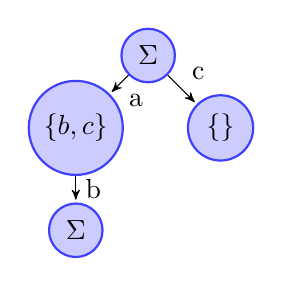
\begin{tikzpicture}[node distance=1.3cm,>=stealth',bend angle=45,auto]
  \tikzstyle{place}=[circle,thick,draw=blue!75,fill=blue!20,minimum size=6mm]
  \tikzstyle{red place}=[place,draw=red!75,fill=red!20]
  \tikzstyle{transition}=[rectangle,thick,draw=black!75,
  			  fill=black!20,minimum size=4mm]
  \tikzstyle{every label}=[red]
  
  \begin{scope}
    \node [place] (w1) {$\Sigma$};
    \node [place] (e1) [below left of=w1] {$\{b,c\}$}
      edge [pre]  node[swap] {a}                 (w1);      
    \node [place] (e2) [below right of=w1] {$\{\}$}
      edge [pre]  node[swap] {c}                 (w1);      
    \node [place] (e3) [below of=e1] {$\Sigma$}
      edge [pre]  node[swap] {b}                 (e1);      
  \end{scope}
    
\end{tikzpicture}
\caption{Example Model}
\label{example model}
\end{figure}
\end{example}

\begin{example}
Figure \ref{threemodels} shows various models of $\MAY{a} \MAY{b}$. 

Because \ELABR{} does not include any of the ``complexifying'' operators $\neg, \lor, $ or $\Rightarrow$, \ELABR{} has the unusual property that every satisfiable formula has a unique (up to isomorphism) simplest model that satisfies it.
In Figure \ref{threemodels}, the left model is the unique simplest model satisfying$\MAY{a} \MAY{b}$.
This property will be used in Section \ref{decisionprocedure} to construct a \emph{linear-time} decision procedure.
\begin{FIGURE}
\centering
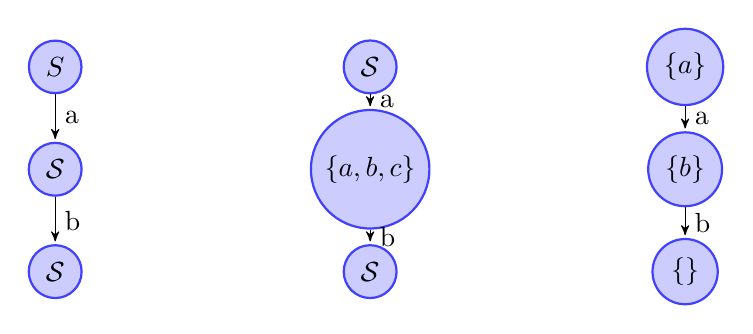
\begin{tikzpicture}[node distance=1.3cm,>=stealth',bend angle=45,auto]
  \tikzstyle{place}=[circle,thick,draw=blue!75,fill=blue!20,minimum size=6mm]
  \tikzstyle{red place}=[place,draw=red!75,fill=red!20]
  \tikzstyle{transition}=[rectangle,thick,draw=black!75,
  			  fill=black!20,minimum size=4mm]
  \tikzstyle{every label}=[red]
  \begin{scope}[xshift=0cm]
    \node [place] (w1) {$S$};
    \node [place] (e1) [below of=w1] {$\mathcal{S}$}
      edge [pre]  node[swap] {a}                 (w1);
    \node [place] (e2) [below of=e1] {$\mathcal{S}$}
      edge [pre]  node[swap] {b}                 (e1);
  \end{scope}   
  \begin{scope}[xshift=4cm]
    \node [place] (w1) {$\mathcal{S}$};
    \node [place] (e1) [below of=w1] {$\{a,b,c\}$}
      edge [pre]  node[swap] {a}                 (w1);
    \node [place] (e2) [below of=e1] {$\mathcal{S}$}
      edge [pre]  node[swap] {b}                 (e1);
  \end{scope}   
  \begin{scope}[xshift=8cm]
    \node [place] (w1) {$\{a\}$};
    \node [place] (e1) [below of=w1] {$\{b\}$}
      edge [pre]  node[swap] {a}                 (w1);
    \node [place] (e2) [below of=e1] {$\{\}$}
      edge [pre]  node[swap] {b}                 (e1);
  \end{scope}   
\end{tikzpicture}
\caption{Various models of $\langle a \rangle \langle b \rangle \top$}
\end{FIGURE}

\end{example}

\begin{example}
Figure \ref{more models} shows one model that does, and one that does not, satisfy the formula $\fBang \{a,b\}$.

\begin{FIGURE}
\centering
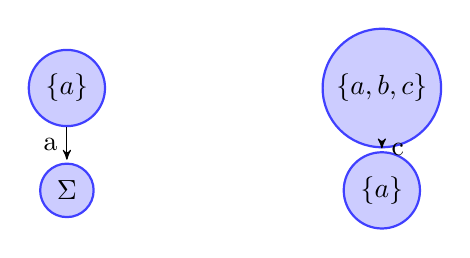
\begin{tikzpicture}[node distance=1.3cm,>=stealth',bend angle=45,auto]
  \tikzstyle{place}=[circle,thick,draw=blue!75,fill=blue!20,minimum size=6mm]
  \tikzstyle{red place}=[place,draw=red!75,fill=red!20]
  \tikzstyle{transition}=[rectangle,thick,draw=black!75,
  			  fill=black!20,minimum size=4mm]
  \tikzstyle{every label}=[red]
  \begin{scope}[xshift=0cm]
    \node [place] (w1) {$\{a\}$};
    \node [place] (e1) [below of=w1] {$\Sigma$}
      edge [pre]  node {a}                 (w1);
  \end{scope}   
  \begin{scope}[xshift=4cm]
    \node [place] (w1) {$\{a, b, c\}$};
    \node [place] (e1) [below of=w1] {$\{a\}$}
      edge [pre]  node[swap] {c}                 (w1);
  \end{scope}   
\end{tikzpicture}
\caption{The model on the left validates $!\{a, b\}$
while the model on the right does not.}\label{figure:elAndBang:moreMdels}
\label{more models}
\end{FIGURE}

\end{example}

\begin{example}
Because \ELABR{} does not include any of the ``complexifying'' operators $\neg, \lor, $ or $\Rightarrow$, the only tautological formulae that are true in all models are $\top$ and conjunctions of $\top$.
But there are an infinite number of distinct contradictory formulae that are false in all models.
For example:
\begin{eqnarray*}
\MAY{a} \land \fBang \{\} \\
\MAY{a} \land \fBang \{b\} \\
\MAY{a} \land \fBang \{b, c\} \\
\MAY{b} \land \fBang \{\} \\
...
\end{eqnarray*}
\end{example}

\begin{definition}
Let $\Gamma$ be an arbitrary set of formulae. We say \emph{$\Gamma$
  semantically implies $\phi$}, written $\Gamma \models \phi$,
provided for all eremic models $\MMM$ if it is the case that $\MMM
\models \Gamma$ implies $\MMM \models \phi$. 
\richard{We do not define $\models \Gamma$ for a set $\Gamma$, only for individual formulae - do we want to change this definition to be of the form $\phi \models \psi$?}
\end{definition}

\begin{example}
\ELABR{} shares with HML the following implications:
\begin{eqnarray*}
\MAY{a} \MAY{b} \models \MAY{a} \\
\MAY{a} (\MAY{b} \land \MAY{c}) \models \MAY{a} \MAY{b}
\end{eqnarray*}
But because \ELABR{} is restricted to deterministic models, it also validates the following formula (which HML does not):
\begin{eqnarray*}
\MAY{a} \MAY{b} \land \MAY{a} \MAY{b}  \models \MAY{a} (\MAY{b} \land \MAY{c})
\end{eqnarray*}
\ELABR{} also validates all implications in which the set of constraints is relaxed from left to right. For example:
\begin{eqnarray*}
\fBang \{\} \models \fBang \{a\} \\
\fBang \{\} \models \fBang \{a, b\} \\
...
\end{eqnarray*}
\end{example}


\section{Capturing Inferences Between Atomic Sentences}
\ELFULL{} arose as an attempt to answer the question: what is the simplest logic that can capture inferences between atomic sentences of natural language? 
In this section, we first enumerate the sorts of inferences we are trying to capture.
Then we show how \ELABR{} can handle these inferences.
Finally, we compare our approach with the various attempts to handle these inferences in First Order Logic.

\subsection{Intra-Atomic Inferences in Natural Language}
Natural language admits many types of inference between atomic sentences.
First, exclusion:
\begin{quote}
``Jack is male'' is incompatible with ``Jack is female''
\end{quote}
Second, entailment inferences from dyadic to monadic predicates:
\begin{quote}
``Jack loves Jill'' implies ``Jack loves''
\end{quote}
Third, adverbial inferences:
\begin{quote}
``Jack walks quickly'' implies ``Jack walks''
\end{quote}
Fourth, inferences from conjunctions of sentences to conjunctions of noun-phrases (and vice-versa):
\begin{quote}
``Jack loves Jill'' and ``Jack loves Joan'' together imply that ``Jack loves Jill and Joan''
\end{quote}
Fifth, inferences from conjunctions of sentences to conjunction of predicates\footnote{See \cite{sommers} p.282 for a spirited defence of predicate conjunction against Fregean regimentation.} (and vice-versa):
\begin{quote}
``Jack is bruised'' and ``Jack is humiliated'' together imply that ``Jack is bruised and humiliated''.
\end{quote}

All these types of inference can be handled directly and naturally in \ELABR{}, as we shall now show.


\subsection{Intra-Atomic Inferences in \ELFULL{}}
We shall show that each of the following inferences can be naturally expressed in \ELABR{}:
\begin{itemize}
\item
``Jack is male'' is incompatible with ``Jack is female''
\item
``Jack loves Jill'' implies ``Jack loves''\footnote{Although natural languages are full of examples of inferences from dyadic to monadic predicates, there are certain supposed counterexamples to the general rule that a dyadic predicate always implies a monadic one. For example, ``Jack explodes the device'' does not, on its most natural reading, imply that ``Jack explodes''. Our response to cases like this is to distinguish between two distinct monadic predicates $explodes_1$ and $explodes_2$:
\begin{itemize}
\item
$X explodes_1$ iff $X$ is an object that undergoes an explosion
\item
$X explodes_2$ iff $X$ is an agent that initiates an explosion
\end{itemize}
Now ``Jack explodes the device'' does imply that ``Jack $explodes_2$'' but does not imply that ``Jack $explodes_1$''. 
There is no deep problem here - just another case where natural language overloads the same word in different situation to have different meanings.}
\item
``Jack walks quickly'' implies ``Jack walks''
\item
``Jack loves Jill'' and ``Jack loves Joan'' together imply that ``Jack loves Jill and Joan''
\item
``Jack is bruised'' and ``Jack is humiliated'' together imply that ``Jack is bruised and humiliated''.
\end{itemize}
First, incompatibility. ``Jack is male'' and ``Jack is female'' are translated into \ELABR{} as the pair of incompatible sentences:
\begin{eqnarray*}
\MAY{jack} \MAY{sex} (\MAY{male} \land \fBang \{male\}) \\
\MAY{jack} \MAY{sex} (\MAY{female} \land \fBang \{female\})
\end{eqnarray*}
Second, entailment from dyadic to monadic predicates:
``Jack loves Jill'' is translated into \ELABR{} as:
\begin{eqnarray*}
\MAY{jack} \MAY{loves} \MAY{jill}
\end{eqnarray*}
This directly entails:
\begin{eqnarray*}
\MAY{jack} \MAY{loves}
\end{eqnarray*}
Similarly, \ELABR{} supports inferences from triadic to dyadic predicates:
\begin{quote}
``Jack passed the biscuit to Mary'' implies ``Jack passed the biscuit''
\end{quote}
This can be expressed directly in \ELABR{} as:
\[
\MAY{jack} \MAY{passed} \MAY{biscuit} \MAY{to} (\MAY{mary} \land !\{mary\}) \models \MAY{jack} \MAY{passed} \MAY{biscuit}
\]
Third, adverbial inferences: 
\begin{eqnarray*}
\MAY{jack} \MAY{walks} \MAY{quickly}
\end{eqnarray*}
entails:
\begin{eqnarray*}
\MAY{jack} \MAY{walks}
\end{eqnarray*}
Fourth, \ELABR{} directly supports inferences from conjunctions of sentences to conjunctions of noun-phrases.
As our models are \emph{deterministic labelled transition systems}, we have the general rule that
\[
\MAY{a} \MAY{b} \land \MAY{a} \MAY{c} \models \MAY{a} (\MAY{b} \land \MAY{c})
\]
from which it follows that 
\begin{eqnarray*}
\MAY{jack} \MAY{loves} \MAY{jill}
\end{eqnarray*}
and:
\begin{eqnarray*}
\MAY{jack} \MAY{loves} \MAY{joan}
\end{eqnarray*}
together imply
\begin{eqnarray*}
\MAY{jack} \MAY{loves} (\MAY{jill} \land \MAY{joan})
\end{eqnarray*}
Using the same rule, we can infer that
\begin{eqnarray*}
\MAY{jack} \MAY{bruised} \land \MAY{jack} \MAY{humiliated}
\end{eqnarray*}
together imply
\begin{eqnarray*}
\MAY{jack} (\MAY{bruised} \land \MAY{humiliated})
\end{eqnarray*}
 
\subsection{Representing Incompatible Predicates in Predicate Logic}
\label{incompatiblepredicatesinfol}
How are incompatible predicates represented in traditional Predicate Logic?
Brachman and Levesque\cite{brachman} introduce the topic of incompatible predicates by remarking:
\begin{quote}
We would consider it quite ``obvious'' in this domain that if it were asserted that $John$ were a $Man$, then we should answer ``no'' to the query $Woman(John)$.
\end{quote}
They propose adding an extra axiom to express the incompatibility:
\[
(\forall x) Man(x) \rightarrow \neg Woman(x)
\]   
This proposal imposes an authoring burden on the knowledge-representer.
We would have to add an extra axiom for every pair of incompatible predicates.
This proposal becomes particularly burdensome when dealing with large sets of incompatible predicates. 
For example, suppose there are 50 football teams, and a person can only support one team at a time. 
We would need to add $C^{50}_2$ axioms:
The incompatibility axioms start to get large and unwieldy:
\begin{eqnarray}
(\forall x) \neg (SupportsArsenal(x) \land SupportsLiverpool(x)) \nonumber \\
(\forall x) \neg (SupportsArsenal(x) \land SupportsManUtd(x)) \nonumber \\
(\forall x) \neg (SupportsLiverpool(x) \land SupportsManUtd(x)) \nonumber \\
... \nonumber
\end{eqnarray}   
Or, if we treat the football-teams as objects, and have a two-place $Supports$ relation between people and teams, we could have:
\[
(\forall x,y,z) \; \; Supports(x,y) \land y \neq z \rightarrow \neg Supports(x,z)
\]   
Together with the Unique Names Assumption (which lets us assume that each football team is distinct from all the others), this certainly captures the desired uniqueness condition.
But it does so by using relatively complex logical machinery.

\subsection{Supporting Inferences from Dyadic to Monadic Predicates in Predicate Logic}
If we want to capture the inference from ``Jack loves Jill`` to ``Jack loves'' in predicate logic, we have to add a non-logical axiom:
\[
(\forall x, y) Loves(x,y) \rightarrow Loves(x)
\]
We would have to add an extra non-logical axiom like this for every n-place predicate.
This is cumbersome at best. 
In \ELABR{}, by contrast, we do not need to introduce any non-logical machinery at all to capture these inferences because they all follow from the general rule that $\MAY{a} \MAY{b} \models \MAY{a}$.

\subsection{Supporting Adverbial Inferences in Predicate Logic}
How can we represent verbs in traditional predicate logic so as to support adverbial inference?
Davidson \cite{davidson2} proposed that every $n$-place action verb be analysed as an $n+1$-place predicate, with an additional slot representing an event.
For example, he  analysed ``I flew my spaceship to the Morning Star'' as 
\[
(\exists x) Flew(I, MySpaceship, x) \land To(x, TheMorningStar)
\]
This implies 
\[
(\exists x) Flew(I, MySpaceship, x)
\]
This captures the inference from ``I flew my spaceship to the Morning Star'' to ``I flew my spaceship''.

Predicate Logic cannot support logical inferences between elementary propositions. 
If it is going to support inferences from adverbial sentences, it \emph{cannot} treat them as elementary propositions and must instead \emph{reinterpret} them as logically complex propositions.
The cost of Davidson's proposal is that a seemingly simple sentence, such as ``Jones walks'', turns out on closer inspection not be elementary at all,  but to involve existential quantification:
\[
(\exists x) Walks(Jones, x)
\]
Although Predicate Logic can handle some of these inferences, it can only do so by reinterpreting the sentences as logically-complex compound propositions. 
It uses more complex machinery to achieve the same results that \ELFULL{} gets directly.

\subsection{Comparison}
We have been looking at five types of inference between atomic sentences:
\begin{itemize}
\item
Incompatibility
\item
Inferences from dyadic predicates to monadic predicates
\item
Adverbial inferences
\item
Inferences from conjunctions of sentences to conjunctions of noun-phrases
\item
Inferences from conjunctions of sentences to conjunctions of predicates
\end{itemize}
\ELFULL{} can handle all five types of inference directly and naturally.
Traditional predicate logic has a harder time.
Traditional predicate logic \emph{can} express incompatibility. But it can only do so by bringing in relatively complex machinery - a universal quantifier, a conditional, and a negation operator. \ELFULL{}, by contrast, expresses the source of the incompatibility \emph{directly} using the $!$ operator.
Again, predicate logic \emph{can} express adverbial inferences. But, again, it can only do so by introducing relatively complex machinery (quantification over events). 

But when it comes to inferences from conjunctions of sentences to conjunctions of noun-phrases (or predicates), predicate logic has nothing to say because it has no way of expressing conjunctions between noun-phrases (or predicates) \emph{at all}. In predicate logic, ``Jack is bruised and humiliated'' has to be regimented into ``Jack is bruised and Jack is humiliated''. 
This might seem, to anyone who has not already become desensitised to the differences between predicate logic and our ergonomic mother tongue, to be exactly the wrong way around.

\subsection{An Expressive Limitation}
As we have seen, \ELFULL{} can handle inferences where predicates are conjoined:
\begin{quote}
``Jack is bruised'' and ``Jack is humiliated'' together imply that ``Jack is bruised and humiliated''.
\end{quote}
It can also handle inferences where predicate-objects are conjoined:
\begin{quote}
``Jack loves Jill'' and ``Jack loves Joan'' together imply that ``Jack loves Jill and Joan''
\end{quote}
But it cannot express related inferences where the \emph{subjects} are conjoined. For example:
\begin{quote}
``Jack loves Jill'' and ``Jim loves Jill'' together imply that ``Jack and Jim love Jill''
\end{quote}
\ELFULL{} has no way to conjoin noun-phrases in subject-position.
We plan to address this representational issue in future work.
\section{Using \ELFULL{} as a Knowledge Representation Language}\label{kr}


\ELFULL{} has been used as the representation language for a large,
complex, highly-dynamic multi-agent simulation \cite{evans-and-short}:
the entire world state is stored as a set of eremic logic formulae -
all other aspects of world state are transient and computed as needed.
The true sentences are represented in a deterministic labeled
transition system, using a non-monotonic update mechanism.  This
application is not a toy problem, but industrial-sized, involving tens
of thousands of rules and equally many atomic facts.  This
demonstrates that eremic logic is a suitable language for representing
complex simulational state.

We shall first sketch how facts are represented, before describing the
advantages of \ELABR{} over a more traditional predicate-logic
representation.

\subsection{Representing facts  in \ELABR{}}

We used the following strategy for representing facts in \ELABR{}.  A
sentence involving a one-place predicate of the form $p(a)$ is
expressed in \ELABR{} as
\begin{eqnarray*}
   \MAY{a} \MAY{p}
\end{eqnarray*}

\NI A sentence involving a many-to-many two-place relation of the form
$r(a,b)$ is expressed in \ELABR{} as
\begin{eqnarray*}
\MAY{a} \MAY{r} \MAY{b}
\end{eqnarray*}
But a sentence involving a many-to-one two-place relation of the form $r(a,b)$ is expressed in \ELABR{}:
\begin{eqnarray*}
\MAY{a} \MAY{r} (\MAY{b} \land \fBang \{b\})
\end{eqnarray*}
So, for example, to say that ``Jack likes Jill'' (where ``likes'' is, of course, a many-many relation), we would write:
\begin{eqnarray*}
\MAY{jack} \MAY{likes} \MAY{jill}
\end{eqnarray*}
But to say that ``Jack is married to Joan'' (where``is-married-to'' is a many-one relation), we would write:
\begin{eqnarray*}
\MAY{jack} \MAY{married} (\MAY{joan} \land \fBang \{joan\})
\end{eqnarray*}

\NI The tranlation is detailed later in Section
\ref{translationFOLtoFOEL}.  Colloquially, we might say that ``Jack is
married to Joan - and only Joan''.  Note that the  relations are
placed in infix position,  so that the facts about an object are
``contained'' within the object.   But we \emph{could}
have chosen an alternative strategy, in which the predicate/relation
symbols are to the left of the first argument. (The reason for
choosing the infix notation will become clear in the next subsection).
 
When applied to a large knowledge base, \ELFULL{} has been found
to have a number of advantages over traditional predicate logic as a
language to represent simulational state:
\begin{itemize}

\item The notion of a sub-tree in \ELABR{} gives us a natural way to
  represent \emph{objects}

\item The update rule (described above) means that \emph{garbage
  collection}\martin{Can we expect readers to understand what that
  means or why it is significant?} of invalid data happens
  automatically.

\item \ELABR{} allows a simpler less error-prone way of specifying
  \emph{postconditions} of actions

\item The $!$ operator gives additional information to the type-checker,
allowing an author to specify her intent more precisely

\item The $!$ operator provides additional information to the
  compiler, allowing significantly more efficient clause ordering

\end{itemize}
We consider  each of these in turn.

\subsection{Using Sub-trees of Expressions to Represent Objects}

\martin{This section is about the algorithmic advantages of
  representing facts as trees, and how EL supports a tree-presentation
  of facts. It's probably an interesting statement about the world
  that it can often be represented in this way.}

\NI Consider the following facts about a gentleman named Brown:
%% \begin{eqnarray*}
%% \MAY{brown} & ( & \\
%% & & \MAY{sex} (\MAY{male} \land \fBang \{male\}) \\
%% & & \MAY{friends} (\MAY{lucy} \land \MAY{elizabeth}) \\
%% & )
%% \end{eqnarray*}

\[
   \MAY{brown} 
   \left(
   \begin{array}{l}
     \MAY{sex} (\MAY{male} \land \fBang \{male\}) \\
        \qquad \AND \\
     \MAY{friends} (\MAY{lucy} \land \MAY{elizabeth}) 
   \end{array}
   \right)
\]
\martin{I have reformated this formula. Is it correct? If not, the old
version is commented out ...}

\NI All the facts which start with the prefix $\MAY{brown}$ form a
sub-tree of the entire database.  And all the facts which start with
the prefix $\MAY{brown} \MAY{friends}$ form a sub-tree of that tree.
A sub-tree can be treated as an individual via its prefix.  The whole
sub-tree can be removed in one fell swoop by deleting its associated
prefix.\martin{Is it clear to the uninitiated reader why this is significant? Shall we relate it to garbage collection mentioned above?}  So we can e.g. remove Brown's friends just by deleting the
sentence $\MAY{brown} \MAY{friends}$.  (Compare this with Prolog\martin{maybe we could structure the kr.tex section as an extended comparison with Prolog. That
might be informative for those readers who know Prolog.} -
where it is much harder to remove all formulae containing a particular
symbol).  A sub-tree of formulae is the \ELABR{} equivalent of an
\emph{object} in an object-oriented programming language.

The tree-structure of formulae also allows us to express the \emph{life-time of data} in a natural way. \martin{this is not about EL as such but about sequences of EL ...}
If we wish a piece of data $d$ to exist for just the duration of a proposition $t$, then we make $t$ be a sub-expression of $d$. 
For example, if we want the friendships of an agent to exist just as long as the agent, then we place the relationships inside the agent: 
\[
\MAY{brown} \MAY{friends}
\]
Now, when we remove $\MAY{brown}$ all the sub-trees, including the data about who he is friends with, will be automatically deleted as well.\martin{does that fall under garbage collection?}

Another advantage of using a tree structure is that we get a form of \emph{automatic currying} which simplifies queries.
So if, for example, Brown is married to Elizabeth, then the database would contain 
\begin{eqnarray*}
\MAY{brown} \MAY{married} (\MAY{elizabeth} \land \fBang \{elizabeth\})
\end{eqnarray*}
In \ELFULL{}, if we want to find out whether Brown is married, we can query the sub-formula directly -  we just ask if 
\begin{eqnarray*}
\MAY{brown} \MAY{married}
\end{eqnarray*}
In traditional predicate logic, if $married$ is a two-place predicate, then we need to fill in the extra argument place with a free variable - we would need to find out if there exists an $X$ such that $married(brown, X)$ - this is slower to compute and more cumbersome to type. 

\subsection{Simpler Postconditions}
\martin{The section heading is not informative, the section could do with an introduction,
because a new subject is started (action planning and execution)}

When expressing the pre- and post-conditions of an action, planners
based on predicate logic\footnote{An early example is STRIPS
  \cite{strips}.} have to explicitly describe the propositions that
are removed when an action is performed:\martin{say why we are using a new font here. What does it signify?}
\begin{verbatim}
action move(A, X, Y)
    preconditions
        at(A, X)
    postconditions
        add: at(A, Y) 
        remove: at(A, X)
\end{verbatim}
Here, we need to explicitly state that when $A$ moves from $X$ to $Y$, $A$ is no longer at $X$. It might seem obvious to us that if $A$ is now at $Y$, he is no longer at $X$ - but we need to explicitly tell the system this. This is unnecessary, cumbersome and error-prone. In \ELFULL{}, by contrast, the exclusion operator means we do not need to specify the facts that are no longer true:
\begin{verbatim}
action move (A, X, Y)
    preconditions
        <A><at>(<X> /\ !{X})
    postconditions
        add: <A><at>(<Y> /\ !{Y})
\end{verbatim}
The ``!" operator makes it clear that something can only be at one
place at a time, and the non-monotonic update rule\martin{We have not
  explained the non-monotonic update rule.  What is it?}
\emph{automatically} removes the old invalid location data.

\subsection{Using the $!$ Operator to Optimize Preconditions}
\label{optimizingpreconditions}
Suppose, for example, we want to find all married couples who are both Welsh.
In Prolog, we might write something like:
\begin{verbatim}
married_couple_at_home(X, Y) :-
    welsh(X),
    welsh(Y),
    spouse(X,Y).
\end{verbatim}	
Rules like this create a large search-space because we need to find all instances of $welsh(X)$ and all instances of  $welsh(Y)$ and take the cross-product \cite{smith-and-genesereth}. If there are $n$ Welsh people, then we will be searching $n^2$ instances of $(X,Y)$ substitutions.

If we express the rule in \ELFULL{}, the compiler is able to use the extra information expressed in the $!$ operator to reorder the literals to find the result significantly faster.
Assuming someone can only have a single spouse at any moment, the rule is expressed in \ELFULL{} as:
\begin{verbatim}
married_couple_at_home * X * Y :-
    <welsh> <X>,
    <welsh> <Y>,
    <spouse> <X> (<Y> /\ !{Y}).
\end{verbatim}	
Now the compiler is able to reorder these literals to minimize the search-space. 
It can see that, once $X$ is instantiated, the following literal can be instantiated without increasing the search-space:
\begin{verbatim}
<spouse> <X> (<Y> /\ !{Y})
\end{verbatim}
The \emph{tantum} operator can be used by the compiler to see that there is at most one $Y$ who is the spouse of $X$.
So the compiler reorders the clauses to produce:
\begin{verbatim}
married_couple_at_home * X * Y :-
    <welsh> <X>,
    <spouse> <X> (<Y> /\ !{Y}),
    <welsh> <Y>.
\end{verbatim}	
Now it is able to find all results by just searching $n$ instances - a significant optimization.
This optimisation has made a significant difference to the run-time cost in our industrial application.







\section{Related Work}

\subsection{Brandom's Incompatibility Semantics}
In \cite{brandom2} and \cite{brandom}, Brandom has emphasised that logical negation is a degenerate case of material incompatibility:
\begin{quote}
Incompatible sentences are Aristotelian \emph{contraries}. A sentence and its negation are \emph{contradictories}. What is the relation between these? Well, the contradictory is a contrary: any sentence is incompatible with its negation. What distinguishes the contradictory of a sentence  from all the rest of its contraries? The contradictory is the \emph{minimal} contrary: the one that is entailed by all the rest. Thus every contrary of ``Plane figure $f$ is a circle'' - for instance ``$f$ is a triangle'', ``$f$ is an octagon'', and so on - entails ``$f$ is \emph{not} a circle''.
\end{quote}
In \cite{brandom}, Chapter 5, Appendix I, Brandom developed a new type of semantics, Incompatibility Semantics, that takes material incompatibility - rather than truth-assignment - as the semantically primitive notion.

Incompatibility Semantics applies to any language, $\mathcal{L}$, given as a set of sentences. 
It uses an incompatibility function $\mathcal{I}$, that, given a set of sentences $S \subseteq \mathcal{L}$, produces the set of sets of sentences that are incompatible with $S$.
We assume that $\mathcal{I}$ satisfies the monotonicity requirement (Brandom calls it ``Persistence''):
\[
\text{If } X \in \mathcal{I}(Y) \text{ and } X \subseteq X' \text{ then } X' \in \mathcal{I}(Y)
\]
Now Brandom defines entailment in terms of the incompatiblity function. Given a set $X \subseteq \mathcal{L}$ and an individual sentence $\phi \in \mathcal{L}$:
\[
X \models \phi \text{ iff } \mathcal{I}(\{\phi\}) \subseteq \mathcal{I}(X)
\]
Now, given material incompatibility (as captured by the $\mathcal{I}$ function) and entailment, he introduces logical negation as a \emph{derived} concept. Using $N \phi$ for the negation of $\phi$, he introduces negation via the rule:
\[
\{N \phi\} \in \mathcal{I}(X) \text{ iff } X \models \phi
\]
Brandom goes on to show that the $N$ operator, as defined, satisfies the laws of classical negation. 
He also introduces a modal operator, again defined in terms of material incompatibility, and shows that this operator satisfies the laws of $S5$.

\ELFULL{} was inspired by Brandom's vision that material incompatibility is conceptually prior to logical negation:
in other words, it is possible for a community of language users to deploy a language including a material incompatibility relation, even if that language has no explicit logical operators such as negation.
The language users of this simple language may go on to introduce logical operators, in order to make certain inferential properties explicit - but this is an optional further development. 
The language before that addition was already in order as it is.

The approach taken in this paper takes Brandom's original insight in a different direction.
While Brandom defines an unusual (non truth-conditional) semantics that applies to any language, we have defined a unusual logic with a standard (truth-conditional) semantics.






\subsection{Other Related work}

Linguists have also investigated how mutually exclusive alternatives
are expressed \cite{OKeeffeA:rouhanocl}\martin{See John C email for
  more precise reference}, but, to the best of our knowledge have not
proposed formal theories of linguistic exclusion.

\PARAGRAPH{Linear logic} Linear logic \cite{GirardJY:linlog,GirardJY:protyp} 
is a refinement of first-order logic and was introduced by
J.-Y.~Girard with the aim of bringing the symmetries of classical
logic to constructive logic. Linear logic has been fruitful in a
variety of fields, in particular in the study of typing systems, where
the concept of linearity puts type-based resource handling on a sound
logical basis.

Linear logic splits conjunction into two: additive and multiplicative
conjunction The former, additive conjunction $A \& B$, is especially
interesting in the context of \ELFULL{}. It can be interpreted
\cite{AbramskyS:comintoll} as an external choice operation in the
terminology of CSP \cite{HoareC:comseq}. External, because the choice
is offered to the environment.  This interpretation has been
influential in the study of types for process calculus,
e.g.~\cite{HondaK:unitypsfsifLONG,TakeuchiK:intbaslaits,HondaK:lanpriatdfscbp}.
Implicitly, additive conjunction gives an explicit upper bound on how
many different options the environment can choose from. For example in
$A \& B \& C$ we have three options (assuming that none of $A, B, C$
can be decomposed into further additive conjunctions).  With this in
mind, and simplifying a great deal, a key difference between $!A$ and
additive conjunction $A \& B$ is that the individual actions in $!A$
have no continuation, while they do with $A \& B$: $!\{l, r\}$ says
that at this point the only available actions are $l$ and $r$. What
happens at later states is not constraind by $!A$.  In contrast, $A \&
B$ says not only that at this point the only available options are $A$
and $B$, but also that if we choose $A$, then $A$ holds 'for ever',
and likewise for choosing $B$. To be sure, the alternatives in $A \&
B$ may themselves contain further additive conjunctions, and in this
way express how exclusion changes 'over time'.

In summary, \ELABR{} and linear logic offer an operator that restricts
the available options. How are they related? Linear logic has an
explicit linear negation $(\cdot)^{\bot}$ which, unlike classical
negation, is constructive. In constrast, \ELABR{} defines a restricted
form negation from $!A$. Can these two perspectives be frutifully
reconciled?

In this context it is also worth noting that like eremic logic, linear
logic has been used for logic programming
\cite{HodasJS:logproiafoill,WinikoffMD:logprowll,PymDJ:uniprotiollp,HarlandJ:prolygao,MillerD:surlinlp}
and as a programming language for narrative generation
\cite{BosserAG:linlogpfng}, see references therein.

\PARAGRAPH{Process calculus} Another formalism that has a form of 
explicit description of mutually exclusive option as a core primitive
are process calculi. They are models of computation based on the idea
of message passing between actors running in parallel. Labelled
transition systems are often used as models for process calculi, and
many concepts, for example bisimulations and Hennessy-Milner logic,
used for developing eremic logic originated from process theory
(although some, such as bisimulation, evolved independently in other
contexts).

Process calculi traditionally have sums, which, in their most general
form, are:
\[
     \sum_{i \in I} P_i
\]
That is a process that can internally choose, or be chosen to evolve
into the process $P_i$ for each $i$. Once the choice is made, all
other options disappear.  Usually, so much generality is not
considered. Instead, input-guarded sums are much better behaved (and
strictly less expressive):
  \[
     \sum_{i \in I} x_{i}(v_i)P_i
  \]
This is a process that can receive a message on each channel $x_i$
and, if such a message arrives with payload $y$, evolve into
$P_i{y/v_i}$ which is the process obtained from $P_i$ by substituting
$y$ for the bound variable $v_i$.  An even better behaved process is
obtained if all inputs use the same input channel and we have only
finitely many alternatives:
  \[
     \sum_{i = 1}^n x(v)P_i
  \]
  Simplifying a great deal, this can be seen as a proof for linear
  logic's additive conjunction
  \[
     \&_{i = 1}^n x(v)A_i
  \]
  provided each $P_i$ is a proof of $A_i$.  It is possible to extend
  the Curry-Howard correspondence to (fragments of) linear logic on
  one side and process calculi on the other \cite{GaySJ:typcalosp}.

In this way, process calculi are related to linear logic (by using
formulae as types) and to eremic logic (because processes and eremic
formulae can be modelled by labelled transition systems, and because
eremic logic is close to logics for processes).\martin{rephrase. How
  did process theory influence EL?}

\PARAGRAPH{Failures/divergences} Our eremic models are remarkably
close to a form of the failures/divergences models that has been used
in the denotational semantics of Hoare's CSP
\cite{HoareC:comseq,RoscoeAW:theapoc}.  In this model, the denotation
of a process $P$ is given as a pair

\[
   (tr, fail)
\]

A \emph{failure} is a pair $(\sigma, R)$ where $\sigma \in \Sigma^*$
and $R \subseteq \Sigma$. The intended interpretation is that a
process $P$ has failure $(\sigma, R)$ provided that $\sigma$ is a
trace of $P$ and after $P$ executes all the actions in $\sigma$ it
refuses to do any action given in $R$. The denotation $\SEMB{P}$ of
$P$ in a failures/divergences model is the the set of all of $P$'s
failures. The set
\[
   traces(P)
      =
   \{ \sigma\ |\ (\sigma, X) \in \SEMB{P} \}
\]
is prefix-closed, hence gives rise of a deterministic labelled
transition system.
\begin{itemize}

\item States are given by the set $traces(P)$ of all traces.

\item Transitions are of the form $\sigma \TRANS{a} \sigma.a$, where
  $\sigma.a$ is the string extending $\sigma$ with the action $a$.

\item Start state is the empty string.

\end{itemize}
We can decorate all states as follows:
\[
   \lambda (\sigma) = \Sigma \setminus R
\]
provided that $(\sigma, R) \in \SEMB{P}$.  Whenever the set $\Sigma$
of symbols is finite, we obtain an eremic model this way.

While the failures/divergences semantics of CSP are somewhat more
complicated due to the possibility of diverging programs, the close
connection between eremic logic and the denotation semantics, as well
as the syntatic similarity with Hennessy-Milner logic suggest that it
might be fruitful to investigate how eremic logic can be used as a
program logic for process calculi.


% \section{Conclusion}\label{conclusion}

We have introduced \Cathoristic{} as a system for capturing logical inferences between the \emph{atomic} sentences of natural language.
Now there have been various attempts to capture these inferences by translating into \fol{}.
We have argued that our translation into \Cathoristic{} is more efficient and more ergonomic, because we are translating into a simple propositional logic - rather than a complex quantificational logic.
We have used \Cathoristic{} as the basis for a logic-programming language that has served in an industrial AI application.

%We thank Marek Sergot, Tom Smith, and Giacomo Turbanti for their thoughtful comments.


\bibliography{../bib} 

\input{inferenceRules}

\end{document}

